\documentclass{article}
\usepackage[utf8]{inputenc}
\usepackage{geometry}
\usepackage{array}
\usepackage{float}
\usepackage{enumitem}
\usepackage{layout}
\geometry{margin=1in}
\usepackage{graphicx}
\usepackage{afterpage}
\usepackage{fancyhdr}
\usepackage{float}
\usepackage{tabularx}
\usepackage{graphicx}


\pagestyle{fancy}
\fancyhf{} 
\lhead{\textit{Ingénierie des panneaux photovoltaïques}} 
\rhead{\thepage}  

\title{Ingénierie des panneaux photovoltaïques}
\author{}
\date{\vspace{-5ex}}
\geometry{margin=1in}
\begin{document}



\maketitle

\begin{center}
    \begin{tabular}{|l|l|}
        \hline
        \multicolumn{2}{|c|}{\textbf{Notions Systèmes - Analyse et conception de systèmes}} \\
        \hline
        \textbf{Version du document} & 1.2 \\
        \hline
        \textbf{Professeur} & Illyas Harti\\
        \hline
        \textbf{Étudiant} & Sami Boufassa\\
                            
        \hline
        \textbf{Date} & 11 Novembre 2024 \\
        \hline
    \end{tabular}
\end{center}

\tableofcontents

\newpage

\section{Angles d'analyse du système cible}
\subsection{Contexte}
La transition énergétique mondiale, marquée par une demande croissante d'énergies renouvelables, soulève des défis majeurs concernant la réduction de la dépendance aux énergies fossiles. Parmi les solutions les plus prometteuses, les systèmes photovoltaïques (PV), qui convertissent l'énergie solaire en électricité, jouent un rôle essentiel dans cette transformation énergétique. Cependant, bien que les technologies photovoltaïques aient fait des progrès considérables ces dernières décennies, plusieurs enjeux techniques, économiques et environnementaux demeurent pour permettre leur déploiement à grande échelle de manière efficace et durable.

Les systèmes photovoltaïques, comprenant principalement des panneaux solaires, sont désormais utilisés dans une large gamme d'applications, allant des installations domestiques aux grandes centrales solaires industrielles. Ces systèmes trouvent leur place dans des secteurs aussi variés que l'habitat, l'industrie, les transports, ou encore les infrastructures publiques, tels que les écoles et les hôpitaux. Ils se déclinent sous diverses formes : centrales solaires, chauffe-eaux solaires, lampadaires photovoltaïques, et bien sûr, les panneaux solaires installés sur des toitures ou des terrains.

La société X spécialisée dans la gestion de data center hébergeant des ordinateurs / serveurs dédiés pour d'autres clients, souhaite installer des systèmes photovoltaïques afin de réduire son empreinte et taxe carbones. Dans ce contexte, l’ingénierie des systèmes photovoltaïques est cruciale pour répondre aux défis de conception, de performance, de coût, et d’intégration dans les réseaux électriques. L’optimisation de ces systèmes nécessite une compréhension approfondie des paramètres techniques et des contraintes environnementales, tout en prenant en compte les aspects économiques et la viabilité à long terme des installations. Cette analyse s'intéresse particulièrement aux panneaux photovoltaïques, leur conception, leur efficacité et leur déploiement dans un réseau de distribution.


\subsection{Système d'intérêt}
Ce système des panneaux photovoltaïques est principalement conçu pour fonctionner dans un environnement industriel, avec une application particulière dans la production d'électricité à partir de l'énergie solaire. Le périmètre du système est clairement défini : il inclut tous les composants physiques nécessaires pour capturer l'énergie solaire et la convertir en électricité. Cela comprend les cellules photovoltaïques, les modules solaires, ainsi que les connexions électriques internes qui permettent la distribution de l'énergie produite. Les panneaux photovoltaïques, bien qu'ils fonctionnent de manière autonome, ne sont pas isolés. Ils doivent être intégrés dans un réseau de distribution d'électricité, ce qui implique des interactions avec d'autres systèmes externes. L'ingénierie de ce système doit donc non seulement modéliser ses constituants, les liaisons entre ses
constituants, mais aussi les relations avec les éléments du milieu extérieur qui définit ses limites. Pour ce faire, après modélisation du périmètre systèmique, l'architecture "trois angles / visions" sera utilisée, comprenant dans un premier temps l'analyse opérationnelle, suivie de l'analyse fonctionnelle, et enfin, de l'analyse organique. Cette démarche d'étude conduit logiqument a un ordonnancement des diagrammes suivants : Diagramme de contexte, diagramme d'états, diagramme de scénario opérationnel, diagramme de scénario fonctionnel, diagramme de scénario organique.








\section{Identification du périmètre systèmique}


\subsection{Milieu extérieur et parties prenantes}
Le système s'insère dans un réseau industriel HTA. En l'occurrence, les panneaux sont utilisés dans des installations de type data center ou bâtiments commerciaux, où l'efficacité énergétique et la réduction des coûts liés à la consommation d'électricité sont des enjeux majeurs. L’optimisation de leur production d’énergie dépend de facteurs externes comme la disponibilité du soleil, la température et l'orientation des panneaux, mais aussi des interactions avec le réseau électrique. L’efficacité du système se trouve ainsi conditionnée par des éléments extérieurs difficilement maîtrisables. 
Afin d'identifier les systèmes et acteurs externes qui interagissent avec le système cible, il est pertinent d'utiliser la méthode des 6W en se posant les questions suivantes :
\begin{itemize}
    \item \textbf{Who ?} : Quelles sont les parties prenantes physiques (humaines ou organisationnelles) qui ont une interaction avec le système ?
    Les acteurs principaux sont les fabricants, les installateurs ou techniciens, les ingénieurs systèmes ou project managers, les gestionnaires de data center, les autorités réglementaires, les utilisateurs finaux autrement dit les fournisseurs d'électricité et les data center, et organismes de certification.
    \item \textbf{What ?} : Quels sont les systèmes externes qui ont une influence sur les missions du système cible?
    \item \textbf{Where ?} : Quelles sont les localisations des systèmes externes qui ont une influence sur le comportement du système ?
    Les lieux où les panneaux photovoltaïques sont installés pour alimenter des systèmes informatiques ou des installations industrielles. Ces centres peuvent être situés dans des zones stratégiques proches de grandes infrastructures électriques.
    \item \textbf{When ?} : Quels sont les systèmes externes qui interagissent tout le temps avec le système ou à certaines périodes seulement ?  L'énergie solaire et les conditions météorologiques (température, humidité et corrosion) influencent la performance des panneaux photovoltaïques en temps réel, avec des variations saisonnières. 
    \item \textbf{Why ?} : Quels sont les systèmes externes qui ont une influence sur la mission ou la raison d’être du système ? Les data center qui utilisent cette énergie pour alimenter leur serveur et les fournisseurs d'électricité qui peuvent racheter l'énergie produite.
    \item \textbf{How ?} : Quels sont les systèmes externes qui ont une influence sur les composants du système cible ? L'énergie solaire détermine en grande partie quel type de semi-conducteur sera utilisé dans la conception des cellules photovoltaïques également affectés par les conditions météorologiques. Le logiciel de monitoring embarqué permettant un suivi en temps réel et l'optimisation de la production d'énergie peut être influencé par les exigences spécifiques du réseau électrique.
\end {itemize}



Chacune de ces parties prenantes a des intérêts et des contraintes spécifiques qui doivent être pris en compte dans la conception et l'exploitation des systèmes photovoltaïques.

Il est à noter que de nouvelles parties prenantes peuvent intervenir au cours du cycle de vie du système selon les évolutions technologiques, réglementaires ou économiques. 
\subsection{Diagramme de contexte} 

Le diagramme de contexte permet de visualiser les interactions entre le système et son environnement, en identifiant les éléments extérieurs qui influent sur le système ou qui sont influencés par lui. Il permet de délimiter le périmètre du système et de définir les interfaces avec les éléments extérieurs. Ici, il a été organisé de manière à positionner respectivement les parties prenantes et systèmes externes, dans les quatre quadrants du diagramme :
\begin{itemize}
    \item \textbf{À gauche} : les entrées du système;
    \item \textbf{À droite} : les sorties du système;
    \item \textbf{En haut} : les principales contraintes ;
    \item \textbf{En bas} : les principales ressources.
\end{itemize} 

\vspace{50pt}
\begin{figure}[H]
    \centering
    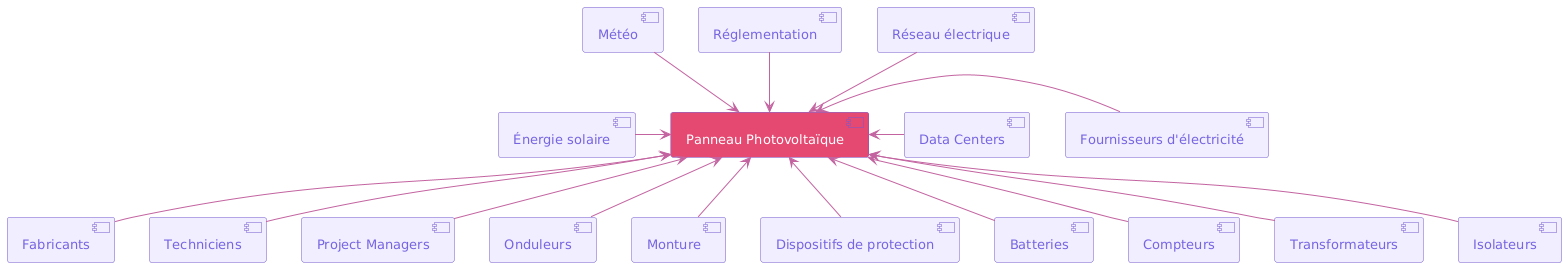
\includegraphics[width=0.95\textwidth]{diagramme_de_contexte.png}
    \caption{Diagramme de contexte du système des panneaux photovoltaïques}
    \label{fig:diagramme_contexte}
\end{figure}
\vspace{10pt}

Le système transforme l'entrée énergie solaire en sortie pour les fournisseurs d'électricité et les data center autrement dit en énergie électrique consommable, à l'aide de l'équilibre du systeme (Balance of System BOS), des fabricants, techniciens et ingénieurs systèmes tout en tenant compte des contraintes environnementales, exigences du réseau et des normes.  



\section{Analyse et modélisation opérationnelle}
\subsection{Expression des besoins}

\subsection{Diagramme de scénario opérationnel}


\section{Analyse et modélisation fonctionnelle}



\subsection{Exigences fonctionnelles}

\clearpage

\subsection{Diagramme d'états}


\subsection{Diagramme de scénario fonctionnel}

\clearpage



\clearpage


\section{Analyse et modélisation organique}



\subsection{Exigences organiques}

\clearpage


\subsection{Diagramme de scénario organique}

\clearpage



\clearpage


\

\section{Annexes}


\end{document}